\section*{Модели циклов}
\addcontentsline{toc}{section}{Модели циклов}
\subsection*{Модель Кейнса}
\addcontentsline{toc}{subsection}{Модель Кейнса}

\textbf{Задание:}\\
Провести численный и качественный анализ модели Кейнса в среде AnyLogic.\\

\textbf{Решение:}\\
$Y$ -- национальный доход (ВВП)\\
$R$ -- процентная ставка\\
$F$ -- разность функции спроса на инвестиции и функции сбережения\\
$L$ -- совокупный денежный спрос\\
$M$ -- постоянное предложение денег

\begin{align*}
	\begin{cases}
		\dfrac{dY}{dt} = \alpha F(Y, R)\\[10pt]
		\dfrac{dR}{dt} = \beta(L(Y, R) - M)\\
	\end{cases}
\end{align*}

Тогда система имеет следующее состояние равновесия:
\begin{align*}
	\begin{cases}
		I(Y, R) = S(Y, R)\\
		L(Y, R) = M\\
	\end{cases}
\end{align*}

Рассмотрим $Y_0$ и $R_0$, которые будут являться решением данной системы.\\

Тогда введём новые переменные и проведём линеаризацию:
\[ u = Y - Y_0 \]
\[ v = R - R_0 \]

\begin{align*}
	\begin{cases}
		\dfrac{du}{dt} = \alpha \dfrac{dF}{dY} u + \alpha \dfrac{dF}{dR} v\\[10pt]
		\dfrac{dv}{dt} = \beta \dfrac{dL}{dY} u + \beta \dfrac{dL}{dR} v\\
	\end{cases}
\end{align*}

\begin{align*}
	\begin{pmatrix}
		\alpha \dfrac{dF}{dY} & \alpha \dfrac{dF}{dR}\\[10pt]
		\beta \dfrac{dL}{dY} & \beta \dfrac{dL}{dR}\\
	\end{pmatrix}
	\longrightarrow
	\begin{vmatrix}
		\alpha \dfrac{dF}{dY} - \lambda & \alpha \dfrac{dF}{dR}\\[10pt]
		\beta \dfrac{dL}{dY} & \beta \dfrac{dL}{dR} - \lambda\\
	\end{vmatrix}
	= 0
\end{align*}

\newpage

\[ \lambda^2 - \lambda \left(\alpha \dfrac{dF}{dY} + \beta \dfrac{dL}{dY}\right) + \alpha \beta \left(\dfrac{dF}{dY} \times \dfrac{dL}{dR} - \dfrac{dF}{dR} \times \dfrac{dL}{dY} \right) = 0 \]

Следовательно:

\[ \lambda_{1,2} = \dfrac{1}{2} \left(\alpha \dfrac{dF}{dY} + \beta \dfrac{dL}{dR} \right) \pm \sqrt{\dfrac{\left(\alpha \dfrac{dF}{dY} + \beta \dfrac{dL}{dR} \right)^2}{4} - \alpha \beta \left(\dfrac{dF}{dY} \times \dfrac{dL}{dR} - \dfrac{dF}{dR} \times \dfrac{dL}{dY} \right)} \]

\[ \dfrac{dL}{dR} < 0,  \dfrac{dF}{dY} > 0, \dfrac{dL}{dY} > 0, \dfrac{dF}{dR} < 0 \]

Таким образом, возможны следующие состояния системы:

\[ \left(\alpha \dfrac{dF}{dY} + \beta \dfrac{dL}{dR} \right) < 0 \]

\[ \alpha \beta \left(\dfrac{dF}{dY} \times \dfrac{dL}{dR} - \dfrac{dF}{dR} \times \dfrac{dL}{dY} \right) > 0 \]

Корни являются комплексными (так как под знаком корня отрицательное число и $\left(\alpha \dfrac{dF}{dY} + \beta \dfrac{dL}{dR} \right) < 0$).\\

$ \lambda_{1,2} = \alpha \pm i \beta, \quad \alpha < 0, \beta \neq 0 $ -- устойчивый фокус

\[ \left(\alpha \dfrac{dF}{dY} + \beta \dfrac{dL}{dR} \right) = 0 \]

\[ \alpha \beta \left(\dfrac{dF}{dY} \times \dfrac{dL}{dR} - \dfrac{dF}{dR} \times \dfrac{dL}{dY} \right) > 0 \]

Корни являются комплексными (так как под знаком корня отрицательное число).\\

$ \lambda_{1,2} = \pm i \beta, \quad \beta \neq 0 $ -- центр

Таким образом, систему уравнений можно переписать следующим образом:

\begin{align*}
	\begin{cases}
		\dfrac{dy}{\alpha dt} = \dfrac{1}{1 + e^{-y}} - l_1 y - r (\beta_1 + \beta_2)\\[10pt]
		\dfrac{dr}{\beta dt} = l_2 y - r \beta_3 - l_s\\
		y(t_0) = y^0, r(t_0) = r^0, y, r > 0\\
	\end{cases}
\end{align*}

\newpage

В соответствии с формулами, данная модель была реализована в среде моделирования AnyLogic. (Рисунок \ref{fig:keins1})
\begin{figure}[h]
	\centering 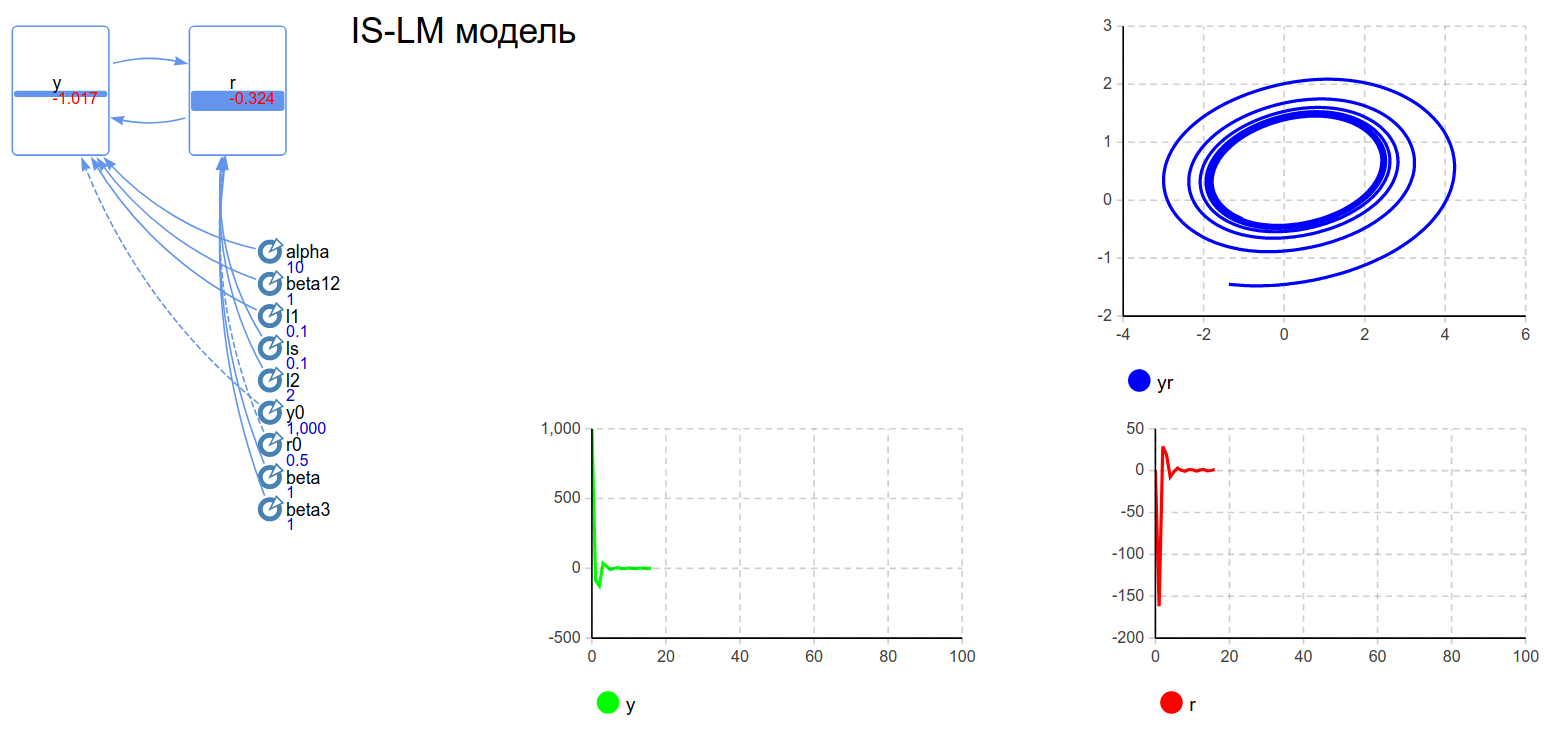
\includegraphics[scale=0.25]{keins1}
	\caption{Результаты построения модели Кейнса в AnyLogic}
	\label{fig:keins1}
\end{figure}

Таким образом, поведение модели, реализованной в AnyLogic, соответствует тому, что было выявлено при качественном анализе модели.\\

Также необходимо было построить модифицированную модель Кейнса. Она может быть представлена следующей системой уравнений:

\begin{align*}
	\begin{cases}
		\dfrac{dy}{\alpha dt} = \dfrac{l_0 K}{l_0 + (K - l_0) + e^{-a_1 y}} - l_1 y - r y (\beta_1 + \beta_2)\\[10pt]
		\dfrac{dr}{\beta dt} = r(l_2 y - r \beta_3 - l_s)\\
		y(t_0) = y^0, r(t_0) = r^0, y, r > 0\\
	\end{cases}
\end{align*}

\newpage

В соответствии с формулами, данная модель была реализована в среде моделирования AnyLogic. (Рисунок \ref{fig:keins2})
\begin{figure}[h]
	\centering 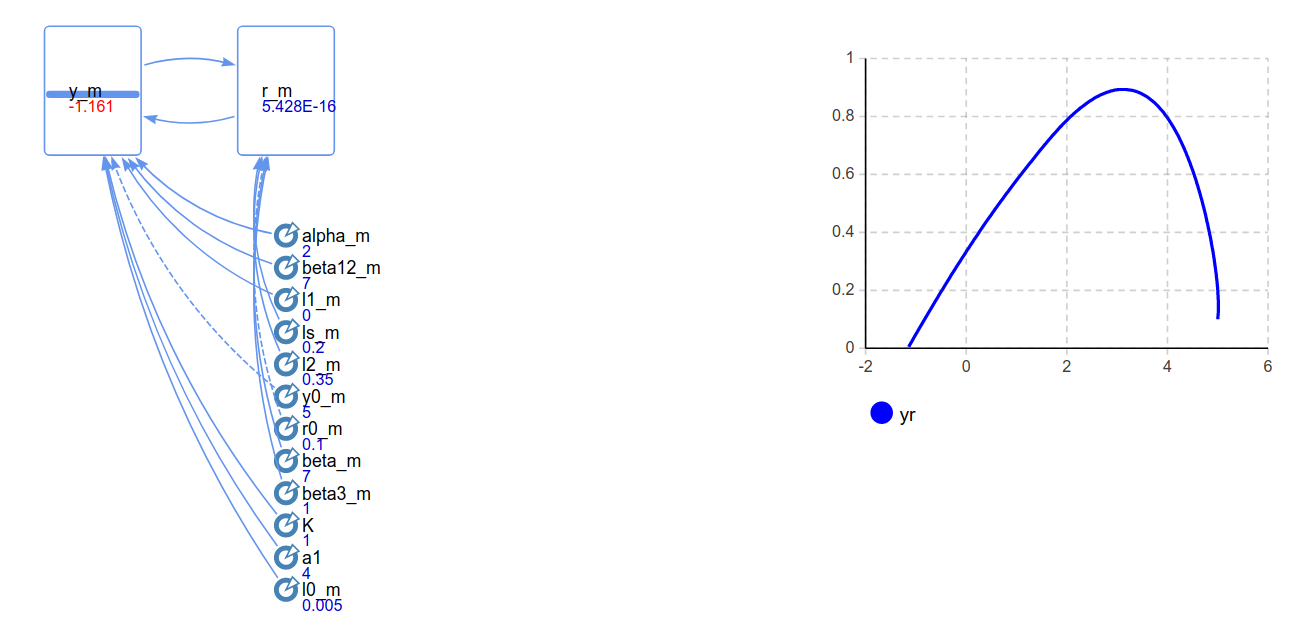
\includegraphics[scale=0.25]{keins2}
	\caption{Результаты построения модифицированной модели Кейнса в AnyLogic}
	\label{fig:keins2}
\end{figure}

Можно видеть, что поведение модели с модифицированной функцией спроса немного изменилось по сравнению с классической моделью, однако в неё по-прежнему сохранился тип равновесия устойчивый фокус и цикл.\\

Таким образом, был проведён численный анализ модифицированной модели Кейнса.\\